\subsubsection{Non-expert User 1 - Brendan}
Brendan is a professor with technological background. They are considered a
non-expert user. An uncontrolled test session was conducted where they tested
each feature of Magpie to find faults, system failures and bugs.

\textbf{Main takeaways from Brendan's session: }Magpie has potential for use by
certain types of users but needs a lot more functionality. Here is a breakdown
of the feedback:
\begin{itemize}
  \item \textbf{Log in/Sign up: } email verification is important, especially
        for a service advertised towards professionals. Also, Brendan did not
        understand the need for username to be created, the username should
        automatically be the email address. As a group, we decided to keep the
        username field as a preference and for future work as the user will be
        greeted by the username chosen when the log in,, or it will display in the
        profile menu.
        \vspace{0.2cm}
        
  \item \textbf{Tutorial: }the content of step 2 needs to be reworked and use
        more descriptive language. Also, the positioning of certain elements is off
        in Firefox browser. For step 4, the word `dozen' should be changed to
        `several' or similar especially if we are planning on adding more amenity
        data. Lastly, step 5 should point to the map, so that is a bug we need to
        investigate bug.
        \vspace{0.2cm}
        
  \item \textbf{Dashboard: }we should implement a button to clear the marker
        and all the points from the map, right now the user is forced to reload the
        page to do that. In addition, it could be beneficial to certain users to
        leave the count of toggled off amenities. Also, compress the list of
        amenities to avoid scrolling. We found Firefox to cause a window size
        issue that we have been unable to address.
        \vspace{0.2cm}
        
  \item \textbf{Map: } plus and minus buttons should be added to zoom in and
        out of the map, especially for users who are not familiar with mouse
        technology. Also, clicking on amenity icons should provide more information.
        Right now, it feels a bit empty. Lastly, some of the selected icons are not
        visually striking, perhaps find a way to emphasize them.
        \vspace{0.2cm}
        
  \item \textbf{Technical: }when clicking on map, there is a slight offset
        between where the marker appears and where the user clicked. There is cause
        for investigation there. Also, maybe think of implementing something to
        avoid mis-clicking and loosing the original marker position.
        
  \item \textbf{Miscellaneous: }Brendan asked why location was being requested
        and what it was used for. Accepting Magpie to use the user's location
        only puts down their own location marker on the map indicating where
        they are located. The location information is not processed by the
        Magpie server, it is processed on the user's device. Additionally, a
        landing page is necessary to present Magpie and put forward the
        machine learning aspect of the project.
\end{itemize}

\textbf{Overall: }the interface is nice, but you might want to focus on
producing a much more data-driven approach for the interface if you want to
attract those kinds of users.

\textbf{Average score from survey: 3.6 out of 5}

\textbf{Score breakdown: Appendix \ref{fig:brendanscore}}

\newpage{}

\subsubsection{Non-expert User 2 - Anonymous 1}
This user has a background in technology at the doctorate level. This session
was mostly uncontrolled, they browsed the application, tested the features and
discussed their thoughts with us.

\textbf{Main takeaways from the session: } this user really enjoyed the
presentation of information on the application, they found the amenities easy to
understand and recognizable in the radius of the map. They tried to interact
with the locked elements of the tutorial, and really enjoyed the confetti at the
end of it. Also, before placing a marker on the map because when they accepted
location tracking, their own marker appeared. To make more improvements, they
suggested the following:
\begin{itemize}
  \item \textbf{More features: }They feel like a search bar would help in the
        quest for information in specific location visually unknown to the user.
        They also though the points would appear automatically on the map but
        instead she had to place her own marker. Perhaps there is an issue with
        onboarding not being retained.
        \vspace{0.2cm}
        
  \item \textbf{Dashboard \& Map: }There is an icon, the water fountain one
        that is neon blue, therefore blends into the white background of the
        dashboard and in the map; probably needs to be changed. Also, more data for
        example on transportation would be a big plus.
        \vspace{0.2cm}
        
  \item \textbf{Miscellaneous: } If you want to appeal to more Non-Expert Users, adding
        more features like location sharing, integrating social interactions and
        make it mobile responsive would be the way to go. Also, a higher level of
        information.
\end{itemize}
\textbf{Overall: }it is a very good application, a very interesting idea to
gather all this information in one place.

\noindent\textbf{Average score from survey: 4.6 out of 5}

\textbf{Score breakdown: Appendix \ref{fig:mairascore}}

\newpage{}

\subsubsection{Non-expert User 3 - Paul}
Our next session was with Paul, a student in technological undergraduate degree.
They gave their contact email in the research survey. A controlled approach was
supposed to be used in this session, however they intuitively went on to explore
the application on their own.

%table of Paul's general tasks
\begin{table}[h!]
  \centering
  \caption{Usability testing Tasks - Paul}
  \begin{tabular}{|p{0.4\textwidth}|p{0.1\textwidth}|p{0.1\textwidth}|p{0.1\textwidth}|p{0.1\textwidth}|}
    \hline
    \textbf{Task}                                 & \textbf{Status} & \textbf{Time taken} & \textbf{Difficulty} & \textbf{Errors}    \\
    \hline
    Load Magpie application                       & Complete        & 20s                 & 1                   & N/A                \\
    \hline
    Sign up                                       & Complete        & 42s                 & 1                   & N/A                \\
    \hline
    Complete tutorial                             & Complete        & 60s                 & 1                   & N/A                \\
    \hline
    Place cursor on map and adjust radius to 250m & Fail            & Skipped             & Skipped             & Skipped            \\
    \hline
    Zoom in to road name level                    & Complete        & 5s                  & 1                   & N/A                \\
    \hline
    Place cursor on another area                  & Complete        & 5s                  & 1                   & N/A                \\
    \hline
    Zoom out to see full radius                   & Fail            & Skipped             & Skipped             & Skipped            \\
    \hline
    Filter to only view "Parking meter" data      & Pass            & 120s                & 3                   & Required help      \\
    \hline
    Filter to toggle off all amenities            & Pass            & 37s                 & 3                   & Required help      \\
    \hline
    Go through tutorial and exit at Step 3        & Pass            & 30s                 & 3                   & Couldn't find icon \\
    \hline
    Log out                                       & Complete        & 20s                 & 2                   & N/A                \\
    \hline
  \end{tabular}
\end{table}

\textbf{Main takeaways from Paul's session: }the map and the amenity data
displayed is `excellent', they would find it useful for local areas of the city.
One aspect they advise we improve on is to make the choice of amenities more
intuitive. This is further supported by their behaviour trying to click on the
icon and amenity title on the dashboard to toggle it on and off, as well as the
difficulties they encountered as shown in the general task table. Another point
to improve on is to make the profile and tutorial icons more visible,
demonstrated by the time they took to find them.

\noindent\textbf{Average score from survey: 4.8 out of 5}

\textbf{Score breakdown: Appendix \ref{fig:paulscore}}

\newpage{}

\subsubsection{Non-expert User 4 - Livia}
Our next session was with Livia, another student in a technological
undergraduate degree  who left their contact in the research survey. This
session also started out as a controlled test with a defined set of tasks, but
just like Paul, Livia went on to explore the application skipping the tasks.

%table of Livias's general tasks
\begin{table}[h!]
  \centering
  \caption{Usability testing Tasks - Livia}
  \begin{tabular}{|p{0.4\textwidth}|p{0.1\textwidth}|p{0.1\textwidth}|p{0.1\textwidth}|p{0.1\textwidth}|}
    \hline
    \textbf{Task}                                 & \textbf{Status} & \textbf{Time taken} & \textbf{Difficulty} & \textbf{Errors} \\
    \hline
    Load Magpie application                       & Complete        & 5s                  & 1                   & N/A             \\
    \hline
    Sign up                                       & Complete        & 16s                 & 1                   & N/A             \\
    \hline
    Complete tutorial                             & Complete        & 44s                 & 1                   & N/A             \\
    \hline
    Place cursor on map and adjust radius to 250m & Complete        & 6s                  & 1                   & N/A             \\
    \hline
    Zoom in to road name level                    & Complete        & 8s                  & 1                   & N/A             \\
    \hline
    Place cursor on another area                  & Fail            & Skipped             & Skipped             & Skipped         \\
    \hline
    Zoom out to see full radius                   & Fail            & Skipped             & Skipped             & Skipped         \\
    \hline
    Filter to only view "Parking meter" data      & Fail            & Skipped             & Skipped             & Skipped         \\
    \hline
    Filter to toggle off all amenities            & Complete        & 18s                 & 1                   & N/A             \\
    \hline
    Go through tutorial and exit at Step 3        & Complete        & 24s                 & 2                   & N/A             \\
    \hline
    Log out                                       & Complete        & 20s                 & 2                   & N/A             \\
    \hline
  \end{tabular}
\end{table}

\noindent\textbf{Main takeaways from Livia's session: }very interesting project,
useful and great; overall a very clear website. Biggest point of discontent for
Livia was the tutorial, they let us know they have dyslexia and the tutorial
could have been worded more effectively to cater to them and others with
learning/visual impediments.

In addition, they tried to interact with the locked elements during the
tutorial, suggesting intuition to put in practice what they are reading to
validate the information absorbed. They also suggested adding more amenities
such as public transports stops, scooter stands and student hubs. They liked how
it was easier to understand the information visually compared to Google maps or
Apple maps.

\textbf{Average score from survey: 4.8 out of 5}

\textbf{Score breakdown: Appendix \ref{fig:liviascore}}

\newpage{}

\subsubsection{Non-expert User 5 - Ben}
Our next test session was with Ben, another student in a technological
post-graduate degree who also left their contact in the research survey. This
session took a more uncontrolled approach and let the users free roam the
application without giving them specific tasks to complete. They were guided
them in the beginning and certain discussions were initiated but overall, the
user was free to explore and think aloud during the process.

%table of Ben's general tasks
\begin{table}[h!]
  \centering
  \caption{Usability testing Tasks - Ben}
  \begin{tabular}{|p{0.4\textwidth}|p{0.1\textwidth}|p{0.1\textwidth}|p{0.1\textwidth}|p{0.1\textwidth}|}
    \hline
    \textbf{Task}                 & \textbf{Status} & \textbf{Difficulty} & \textbf{Errors} \\
    \hline
    Load Magpie application       & Complete        & 1                   & N/A             \\
    \hline
    Sign up                       & Complete        & 1                   & N/A             \\
    \hline
    Log in                        & Complete        & 1                   & N/A             \\
    \hline
    Complete tutorial             & Complete        & 1                   & N/A             \\
    \hline
    Place cursor on map           & Complete        & 1                   & N/A             \\
    \hline
    Zoom in and out               & Complete        & 1                   & N/A             \\
    \hline
    Hold map and navigate         & Complete        & 1                   & N/A             \\
    \hline
    Adjust radius big/small       & Complete        & 1                   & N/A             \\
    \hline
    Clear marker \& radius        & Skipped         & Skipped             & Skipped         \\
    \hline
    Deselect all amenities        & Complete        & 1                   & N/A             \\
    \hline
    Select one or more amenities  & Complete        & 1                   & N/A             \\
    \hline
    Find tutorial and exit midway & Skipped         & Skipped             & Skipped         \\
    \hline
    Log out                       & Complete        & 1                   & N/A             \\
    \hline
  \end{tabular}
\end{table}

\noindent\textbf{Main takeaways from Ben's session: }the application does
exactly what we described it to do- a GIS application to give a at a glance of
amenities in Dublin. The overall impression is that it is a very helpful
application, easy to use and effective. Points to improve are the loading times
for the amenity points, perhaps directly being logged in after sign up to avoid
repetitive steps, make the profile and tutorial icons more visible as they blend
into the map, remove mac keyboard icons from the profile bubble, and if possible
add more information on each amenity perhaps with tooltips, or add more amenity
data like public transportation.

\textbf{Average score from survey: 4.6 out of 5}

\textbf{Score breakdown: Appendix \ref{fig:benscore}}

\newpage{}

\subsubsection{Non-expert User 6 - Jakub}
Jakub is a professional with a construction and technological background. They
were recruited towards the end of product development to test Magpie. This was
an uncontrolled test session where Jakub discovered the application on their
own, discussing each feature, testing each feature, and were then given a small
scenario `Put yourself in the shoes of an urban planner\ldots' to obtain a
different kind of feedback from previous sessions.

%table of Jakub's general tasks
\begin{table}[h!]
  \centering
  \caption{Usability testing Tasks - Jakub}
  \begin{tabular}{|p{0.4\textwidth}|p{0.1\textwidth}|p{0.1\textwidth}|p{0.1\textwidth}|p{0.1\textwidth}|}
    \hline
    \textbf{Task}                 & \textbf{Status} & \textbf{Difficulty} & \textbf{Errors}    \\
    \hline
    Load Magpie application       & Complete        & 1                   & N/A                \\
    \hline
    Sign up                       & Complete        & 1                   & N/A                \\
    \hline
    Log in                        & Complete        & 1                   & N/A                \\
    \hline
    Complete tutorial             & Complete        & 1                   & N/A                \\
    \hline
    Place cursor on map           & Complete        & 1                   & N/A                \\
    \hline
    Zoom in and out               & Complete        & 1                   & N/A                \\
    \hline
    Hold map and navigate         & Complete        & 1                   & N/A                \\
    \hline
    Adjust radius big/small       & Complete        & 1                   & N/A                \\
    \hline
    Clear marker \& radius        & Pass            & 3                   & Did not see button \\
    \hline
    Deselect all amenities        & Complete        & 1                   & N/A                \\
    \hline
    Select one or more amenities  & Complete        & 1                   & N/A                \\
    \hline
    Find tutorial and exit midway & Skipped         & Skipped             & Skipped            \\
    \hline
    Log out                       & Complete        & 1                   & N/A                \\
    \hline
  \end{tabular}
\end{table}
\noindent\textbf{Main takeaways from Jakub's session: }this tool simplifies the
search for amenities however there are certain items that need to be considered
to improve the application:

\begin{itemize}
  \item \textbf{Log in/Sign up: }Email verification should be included, so
        that the user can confirm they have successfully signed up and also for
        security purposes.
        \vspace{0.2cm}
        
  \item \textbf{Map: }some of the amenity data doesn't have accurate
        locations, for example public toilets seem to be off by longitude, and
        multi-storey parking data seems incomplete. Also, water fountains are very
        hard to find on the map, we should consider changing its colour. Same with
        the profile and tutorial icon, they are hard to spot on the map. They would
        also like to double click on the map to clear it, more intuitive for them.
        And last thing, amenities with small count are hard to find in the radius,
        maybe make them more visible somehow.
        \vspace{0.2cm}
        
  \item \textbf{History feature: }doesn't see the use for a non-expert user,
        and again same for this tool, doesn't see the use for them as a non-expert
        user but could be useful for a target user.
        \vspace{0.2cm}
        
  \item \textbf{Extra features: }Search functionality would be very useful for
        those that are looking for a spot but don't know where it is located
        visually. Also, an export feature would be useful for the scenario of urban
        planning, if I'm to put a report together, a visual from this tool would be
        helpful for illustration.
\end{itemize}

\newpage{}

A notable behaviour indicator from them was that they tried to interact with the
elements during onboarding, as have previous users. Due to technical
limitations, we have been unable to make that happen. Future work.
Overall, the tooltips for the icons is very interesting, a suggestion would be
to add the type of parking, zoning information and tariff to the car parking
amenity.

\textbf{Average score from survey: 4.6 out of 5}

\textbf{Score breakdown: Appendix \ref{fig:jakubscore}}

\subsubsection{Non-Expert User Summary}
Non-Expert Users provided very valuable feedback throughout the usability testing
phase of the project. New features have been implemented, reviewed and removed
thanks to these sessions.
For example, zoom buttons were added, tooltips were implemented and icons were
changed. Most notable points raised during these sessions have been the want for
more high level information on the amenities, more amenity data, the visual
feedback from the system when it is loading the points and the onboarding.

The average success rate and average difficulty of a task has been computed in
the table below. The average success rate has been calculated based on the
values of task success, \emph{complete} = 1, \emph{pass} = 0.5 or \emph{fail} =
0.
The average difficulty has been calculated based on the values of task
difficulty from 1 = Easy to 5 = Difficult.

\begin{table}[h!]
  \centering
  \caption{Usability testing Tasks - Non-Expert Users Summary}
  \begin{tabular}{|p{0.4\textwidth}|p{0.2\textwidth}|p{0.2\textwidth}|}
    \hline
    \textbf{Task}                 & \textbf{Task Success Rate} & \textbf{Average Difficulty} \\
    \hline
    Load Magpie application       & 100\%                      & 1                           \\
    \hline
    Sign up                       & 100\%                      & 1                           \\
    \hline
    Log in                        & 100\%                      & 1                           \\
    \hline
    Complete tutorial             & 100\%                      & 1                           \\
    \hline
    Place cursor on map           & 100\%                      & 1                           \\
    \hline
    Zoom in and out               & 100\%                      & 1                           \\
    \hline
    Hold map and navigate         & 100\%                      & 1                           \\
    \hline
    Adjust radius big/small       & 100\%                      & 1                           \\
    \hline
    Clear marker \& radius        & 50\%                       & 3                           \\
    \hline
    Deselect all amenities        & 87.5\%                     & 1.5                         \\
    \hline
    Select one or more amenities  & 87.5\%                     & 1.5                         \\
    \hline
    Find tutorial and exit midway & 75\%                       & 2.5                         \\
    \hline
    Log out                       & 100\%                      & 1.5                         \\
    \hline
  \end{tabular}
\end{table}

Users struggled to find the icons in the beginning to log out or go through the
tutorial again, as well as the button to clear the radius and points from the
map. Almost all Non-Expert Users skipped the "Clear marker and radius task",
showing that they either did not notice it or did not have a use for it.

\newpage{}

To conclude, Non-Expert Users gave Magpie a score of \underline{4.5 out of 5}.
%general survey score summary
\begin{figure}[h!]
  \centering
  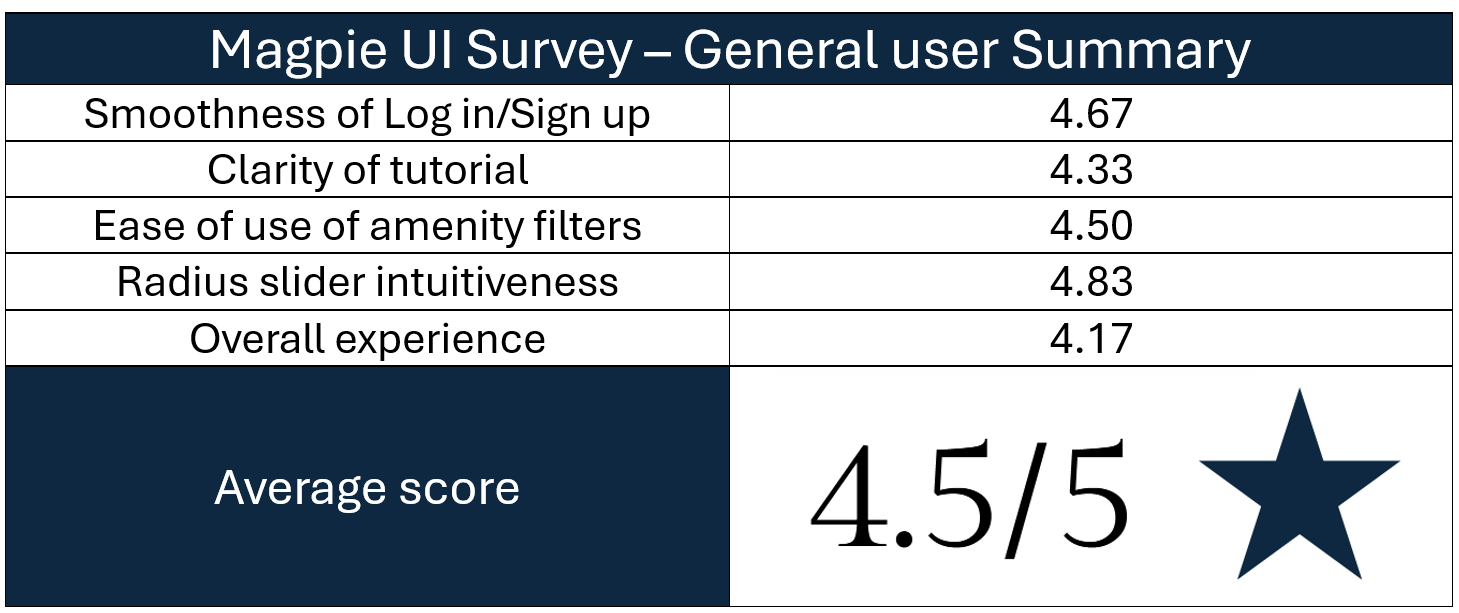
\includegraphics[width=0.7\textwidth]{images/survey-casual-summary.png}
  \caption{User Evaluation - UI General Score Average}
\end{figure}

There was no notable increase in score as the user evaluation progressed between
the users, except in the beginning from the session with Brendan where we scored
\underline{3.6 out of 5} to the session with Anonymous 1 where we scored
\underline{4.6 out 5}. Both users experienced the same version of Magpie, so the
difference in score could come down to one personal preference.